\section{Audio Signal Generators (ASG)}
\label{sect:ASG}
Included with the "Audio Test Instrument" firmware expansion were three signal generators and a fourth Gaussian White Noise generator. These four signals are summed, if turned on, and appear at the left or "impedance" terminals.  These are for general use, but not available when the AVNA Network Analyzer instrument is operating, i.e., when impedance or transmission measurements are being made.  The Signal Generators can produce sine waves or square waves all under direct control of the touch screen.  In addition, under USB serial control this capability  expanded to other waveform types, such as triangles (described in Section \ref{subsect:SerDes}).

Frequencies can be set from 10 to 40,000 Hz in 1 Hz steps, on-screen.  The amplitude is specified by the peak-to-peak value in volts.  The output impedance is 50-Ohms
%
\footnote{50-Ohms applies to the left measurement terminals.  A low impedance output of perhaps 1 Ohm is available at the BNC connector.  Either output can be used used.  }
%
 and the voltage displayed is that delivered to a 50-Ohm load. When open-circuited, the voltage will be double the displayed value.  For convenience, there is provision to turn each generator on and off while leaving the settings alone.

% \subsection{Description}
%MOVE/DELETE   >>>>>>>>>>>>>>>>>>>>>>>>>> 
%A couple of minor corrections.  In the example, the comments on the SigGen settings have the wrong amplitude levels.   The commands are OK.  The correct comments are \\ \\
 %\texttt{SIGGEN 1 1 1234.56 0.1 3}  // SG \#1 as a triangle wave 0.1 v p-p \\
 %\texttt{SIGGEN 4 1 0.0 0.003 0}  // SG \#4 Gaussian White Noise, $\sigma = 0.003$\\

\subsection{Instructions}
\label{subsect:ASGInstr}
As usual, we start with the Home screen of Figure  \ref{AVNA_000-label}.    Tapping on the button, "Signal Gens" brings up a Signal Generator summary screen such as seen here in Figure \ref{AVNA_021-label}.  This shows the frequency, voltage setting, on/off status and waveform for the three signal generators.  A fourth line is for the Gaussian White Noise generator and the frequency for this is never adjustable.  When a generator is off, the on/off status appears in the pinkish color.  The control function of this screen is to allow bringing up one of four control screens for the individual generators.  We continue this by tapping on the "SigGen 1" button on the bottom row.
%
\begin{figure}[H]
\begin{center}
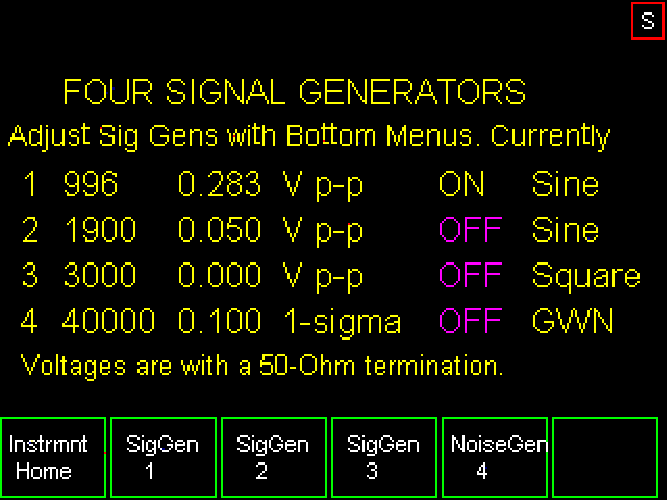
\includegraphics[scale=0.75]{./images/AVNA_021.pdf}
\caption{Signal Generator summary screen. }
\label{AVNA_021-label}
\end{center}
\end{figure}
%
This brings up Signal Generator \#1 control screen as seen in Figure  \ref{AVNA_022-label} below.
%
\begin{figure}[H]
\begin{center}
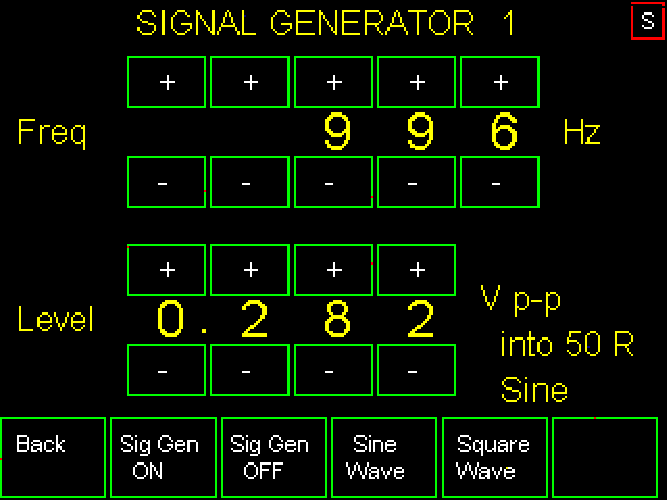
\includegraphics[scale=0.75]{./images/AVNA_022.pdf}
\caption{Signal Generator \#1 control screen  showing a 996 Hz sine wave at 0.282 Volts, p-p.  }
\label{AVNA_022-label}
\end{center}
\end{figure}
%
Here we see plus and minus buttons to control the individual digits for both frequency and amplitude.  In addition, we can turn this generator on and off with the "SigGen ON" and "SigGen OFF" buttons.  To the right of those buttons are a pair for selection of waveform, "Sine Wave" or "Square Wave."  You can make any of those changes now and then use the Back" button to return us to the Signal Generator summary screen, Figure \ref{AVNA_021-label}.

Assuming that you have returned to the summary screen, you can tap on the "NoisGen 4" button to bring up that control screen, Figure  \ref{AVNA_024-label}.
\begin{figure}[H]
\begin{center}
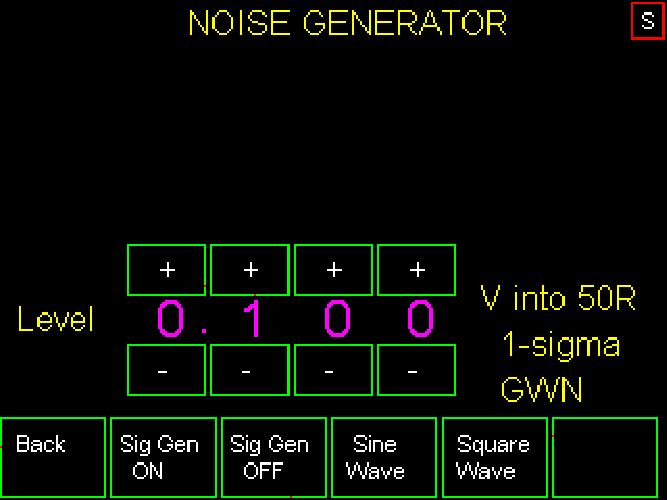
\includegraphics[scale=0.75]{./images/AVNA_024.pdf}
\caption{Gaussian White Noise generator with the 1-sigma value (standard deviation) set to 0.100 Volts when running into a 50-Ohm load.  The pinkish color of the 1-sigma value indicates that the noise generator is currently turned off.}
\label{AVNA_024-label}
\end{center}
\end{figure}
%
This Noise Generator control is basically the same as the Signal Generators, except that there is no frequency control.  The spectrum of the noise is always flat, almost up to half the sample frequency, as set by the Spectrum Analyzer.  This is discussed further below.

\subsubsection{Signal Generator Waveforms}
\label{subsect:ASGWaveforms}
For sine waves, the waveform is excellent up to about 5/12th of the sample frequency, above which the amplitude drops off.   That corresponds to 40 kHz for the highest 96 kHz sample frequency.  For non-sine waves like our square wave, harmonics of the fundamental frequency are needed to build the waveform.  The missing high frequency pieces due to our limited band, cause the waveform to be distorted.  For waveforms like the square wave, this can be an important limitation and suggests keeping the generator frequency far below half the sample frequency, if possible. 
%
\footnote{For a more thorough treatment of the construction of a square waveform a sine wave and odd harmonics, see  \linebreak \textbf{\texttt{https://mathworld.wolfram.com/FourierSeriesSquareWave.html}}. \linebreak  The graph shows the result of limiting the spectrum to the fundamental, fundamental plus third harmonic, and fundamental plus third and  fifth harmonics.  The result gets closer with more harmonics, but the process requires many harmonics to not have obvious distortion. }
%
 In general, it pays to look at the waveform on an oscilloscope if the details are important.

If 3 sine waves are turned on at once, there can be times when all three will add together for a maximum voltage.  The sum of the three voltage settings should therefore be kept below the overload point of about 0.6 volts.

Note that all the control of the Signal Generators is also available from the Serial control using the USB plug.  Also note that over the Serial path the frequency can be controlled to the miliHertz, amplitude to the microVolt and the selections there also include triangle and two sawtooth waveforms.

\subsubsection{Noise}
\label{subsect:ASGNoise}
Signal  Generator \#4 produces Gaussian White noise.  There is an amplitude setting that corresponds to the 1-sigma voltage.  This is a convenient descriptor since the noise power is this voltage squared and divided by 50.  Being "White" noise, the power is spread uniformly across the band  of 0 to half the sampling frequency.  This means that the noise power density is the total noise power divided by half the sampling frequency,  expressed in Watts per Hz.  Keep in mind that the sampling frequency can be changed by the Spectrum Analyzer.
 For instance, if the 1-sigma noise level is 0.1 Volts, the power delivered to a 50-Ohm load is $0.1^2/50 = 0.0002$ Watts (0.2 milliWatts).   If the sample rate is 12 kHz the power is spread across 6 kHz so the power density is 0.2/6000 = 0.0000333 mW/Hz.  In dBm terms, this is -44.8 dBm/Hz.  As seen on the spectrum analyzer, with a noise bandwidth (for this sample rate) of 17.6 Hz, this will show about 17.6 * 0.0000333 = 0.000587 milliWatts per bin, or in dBm terms -32.3 dBm per bin.   This type of arithmetic allows setting the noise generator and the signal generators for any desired situation.

An interesting issue with this noise generator is to find the voltage setting that prevents overload, since Gaussian noise theoretically has no limit and the generator used here can achieve 12 times the 1-sigma voltage.  If you are looking for a high level of noise output, it is reasonable to set the 1-sigma point at 0.1 Volts overload (5-sigma = 0.50 Volts). For a 96 kHz sample rate, this will overload about every 20 seconds, on the average.  This will not be important for most experiments.
